% This project is part of the stellarTwins project.
% Copyright 2017 the authors.

%@archiver{PUT FIGURE NAME HERE}

% # To-do list
% - We need a standard name for the \tgas--\tmass--\PanSTARRS\ Intersection.
% - zeroth draft / re-write the method section
% - add ORCIDs like Hogg's

\documentclass[modern]{aastex61}
\usepackage{amsmath}
\setlength{\parindent}{\baselineskip} % trust me!
\renewcommand{\twocolumngrid}{} % trust me!

% text macros
\newcommand{\foreign}[1]{\textsl{#1}}
\newcommand{\acronym}[1]{{\small{#1}}}
\newcommand{\project}[1]{\textsl{#1}}
\newcommand{\tgas}{\project{\acronym{TGAS}}}
\newcommand{\tmass}{\project{\acronym{2MASS}}}
\newcommand{\gaia}{\project{Gaia}}
\newcommand{\panstarrs}{\project{Pan\acronym{STARRS}}}
\newcommand{\xd}{\acronym{XD}}
\newcommand{\cmd}{\acronym{CMD}}

% math macros
\DeclareMathOperator*{\argmax}{arg\,max}
\newcommand{\given}{\,|\,}
\newcommand{\true}{\mathrm{true}}

% start and title
\shorttitle{improving gaia parallaxes}
\shortauthors{anderson et al.}
\begin{document}\sloppy\sloppypar\raggedbottom\frenchspacing % trust me
\title{Improving \textsl{Gaia} parallaxes
       with a data-driven model \\
       of the color--magnitude diagram}

\author[0000-0001-5725-9329]{Lauren Anderson}
\affil{Center for Computational Astrophysics, Flatiron Institute, 162 Fifth Ave, New York, NY 10010, USA}

\author[0000-0003-2866-9403]{David W. Hogg}
\affil{Center for Computational Astrophysics, Flatiron Institute, 162 Fifth Ave, New York, NY 10010, USA}
\affil{Center for Cosmology and Particle Physics, Department of Physics, New York University, 726 Broadway, New York, NY 10003, USA}
\affil{Center for Data Science, New York University, 60 Fifth Ave, New York, NY 10011, USA}
\affil{Max-Planck-Institut f\"ur Astronomie, K\"onigstuhl 17, D-69117 Heidelberg}

%\author{Jo Bovy}
%\affil{Center for Computational Astrophysics, Flatiron Institute, 162 Fifth Ave, New York, NY 10010, USA}
%\affil{Department of Astronomy and Astrophysics, University of Toronto, 50 St. George Street, Toronto, ON M5S 3H4, Canada}

%\author{Boris Leistedt}
%\affil{Center for Cosmology and Particle Physics, Department of Physics, New York University, 726 Broadway, New York, NY 10003, USA}

%\author{Adrian Price-Whelan}
%\affil{Princeton University Observatory, Princeton University, 4 Ivy Lane, Princeton, NJ 08544, USA}

\begin{abstract}\noindent % trust me

Conversion of a noisy parallax measurement into a posterior belief over distances requires inference with a prior.
Usually this prior represents some kind of belief about the Milky Way.
However, there is multi-band photometry for a large fraction of the \gaia\ \tgas\ catalog from imaging surveys;
this imaging is incredibly informative about stellar distances.
Here we use color information of $1.2$ million \tgas\ stars from \tmass\ to build a noise-deconvolved empirical prior distribution for stars in color--magnitude space.
This data-driven model contains no knowledge of the physics of stellar interiors or photospheres, nor of the Milky Way, but rather derives its precision from its generative model of noisy parallax measurements and an assumption of stationarity.
We use the Extreme Deconvolution (\xd) algorithm, which is an Empirical Bayes approximation to a full hierarchical model of the true parallax and photometry of every star.
The algorithm is run not in absolute-magnitude space but in a transformed space where the measurement uncertainty is closer to Gaussian.
The \xd-optimized prior is used to perform parallax inferences for every star, yielding a precise photometric parallax estimate and uncertainty (and full posterior) for every star.
Our posterior photometric parallax estimates are more precise than the \tgas\ catalog entries by a median factor of [XXX]; and more precise than previous examples of Bayesian distance estimates by a factor of [YYY].
%The precision can be attributed to the statistics concept of shrinkage.
We independently validate our distances by looking at members of a Milky Way star cluster M67, which is not visible as a cluster in the \tgas\ parallax estimates, but appears clearly as a cluster in our posterior parallax estimates.
All our results, including a posterior parallax and distance sampling for [ZZZ] \tgas\ stars, are available in companion electronic tables.
\end{abstract}

\keywords{
  catalogs
  ---
  Hertzsprung--Russell and C--M diagrams
  ---
  methods: statistical
  ---
  parallaxes
  ---
  stars: distances
  ---
  stars: statistics
}

\section{Introduction}

The \gaia\ Mission (\citealt{gaia16}) will deliver more than a billion stellar parallax measurements.
Only a small fraction (but large number) of these
measurements will be both precise and purely astrometric.
\gaia\ will use astrometric parallax to determine the distances of the more precise
stars, and then calibrate spectrophotometric models.
These spectrophotometric models, in turn, along with \gaia's on-board
low-resolution $B_p\,R_p$ spectrophotometry, are used to provide
parallax estimates to less precise stars.
The full stack required for these parallax inferences is complex.
It involves modeling the stars, as well as the dust in the Milky Way,
and the response of the telescope itself.
It might be possible to eliminate some of this complexity using data driven models which don't rely on physical models.

Projects like \project{The Cannon} (\citealt{ness15}; \citealt{casey17}; \citealt{ho17})
and \project{Avast} (Bedell et al.\ in preparation),
explore the extent to which our predictive models of
stars could be purely data-driven or statistical.
That is, under what circumstances could the data themselves deliver
more precise or more accurate information than any theoretical or
physics-based model?
The answer to this question is extremely context-dependent: It depends
on what data are available, how much data are available, and what
questions are being asked.
In general, data-driven models contain fewer assumptions than
physics-driven models, but they are also usually less interpretable.
However, the \gaia\ data set is ideal for thinking about purely statistical
models of stars:
The distance to a star is a latent variable, and the nearby
stars constitute a high signal-to-noise ``training set''.
These nearby stars can be used to anchor empirical models that can
then be applied to the more distant stars.

Here we deliver a demonstration-of-concept that shows that a
data-driven model of the \gaia\ data could in principle deliver very
precise parallaxes, without any input of the physics or numerical models of stellar
evolution, interiors, or photospheres.
HOGG:What is a photometric parallax? <Enter here>
Most stellar models used to generate photometric distances or photometric
parallaxes have been physical models, based on gravity, fluid mechanics,
radiative transfer, nuclear reactions, and atomic and molecular transitions.
Because there are small issues with each of these components, the models are inaccurate in detail, and
the physical models therefore produce distance estimates that are biased.
In addition, they build a long list of physical assumptions (about
nuclear reactions, convection, and thermal timescales, for example)
into the parallax estimates.
When using physical models, it is impossible to deliver photometric parallax estimates that involve minimal assumptions.

However, the use of physical models for distance estimation is not necessary.
It is possible to build a stellar photometric model from the data themselves,
because there are stars at all luminosities with useful parallax information,.
One challenge is that different stars are observed at different levels of parallax precision,
so it requires relatively sophisticated technology to build this data-driven model
using all the data available, fairly and responsibly.
Luckily, we have this technology!

Here we build and use just such a data-driven model to infer more precise parallaxes for each star.
In particular, we use all of the \gaia\ \tgas\ data (\citealt{tgas};
these data were generated by the methodology of \citealt{michalik15}), that match to the
\tmass\ photometry (\citealt{skrutskie06}) and lie in the footprint of
the \panstarrs\ Dust Map (\citealt{green15}), to make a model of the
noise-free (or low-noise) color--magnitude diagram (\cmd) of stars.
We build the \cmd\ using an Empirical-Bayes approach known as Extreme Deconvolution (XD;
\citealt{bovy11}).
This method deconvolves heteroskedastic data to derive an
estimate of the noise-free or low-noise distribution that \emph{would
  have} been observed with far better data.
This method has been used in astrophysics
previously to model the velocity distribution of stars in the Solar
Neighborhood (\citealt{hogg05}; \citealt{bovy09}) and to
perform quasar target selection
in \project{Sloan Digital Sky Survey} data (\citealt{xdqso}; \citealt{xdqsoz}).
Its advantage over other deconvolution methods is that it takes as input,
and handles in a principled way, heteroskedastic data.
Its disadvantage, for the present purposes, is that it requires
or implies a strictly Gaussian noise model.
As we show below, this requires us to transform the \cmd\ to a space in which
the noise is approximately Gaussian.

We then use the novel \xd\ output---the deconvolved \cmd---as
a prior for use in inference of individual-star parallaxes.
These inferences, one per star, provide much more precise parallax, distance,
or absolute magnitude estimates than we get from each star's primary
\tgas\ parallax measurement alone.
That is, we are using the \xd\ model to de-noise the \gaia\ parallax
measurements.
Technically, since \xd\ produces a maximum-marginalized-likelihood estimator
of the deconvolved distribution,
its use as a prior is technically using the data twice and is therefore only approximately valid.
However, since the data set is large, the \xd\ approximation is not bad; it is
sometimes known as the ``empirical Bayes'' method, and is well studied\footnote{For a start, try \url{https://en.wikipedia.org/wiki/Empirical_Bayes_method}.}.

It wouldn't be using the data twice---that is, it would be valid from a
probabilistic perspective---if we performed a full hierarchical Bayesian
inference.
Exploration of that possibility, and its computational tractability,
is among our long-term goals and motivations.
Along those lines, this paper can be seen as a companion to a related
project (Leistedt et al. in preparation), in which we use a slightly less appropriate
model for the \cmd, but in which we take a much more principled
approach to the inference.

Although not a fully Bayesian hierarchical inference, the methodology presented in this paper makes exceedingly weak assumptions
about the Milky Way, and similarly weak assumptions about the properties of
stars.
To date, there has been some discussion in the literature
about how to use a parallax responsibly to infer a distance (\citealt{astraatmadja16a}; \citealt{astraatmadja16b}).
These papers use the \gaia\ measurement to construct a parallax likelihood,
and combine this with a distance prior.
While this is sensible and correct, all present methods proposed along
these lines build in informative (and known-to-be-wrong) assumptions
about the line-of-sight distance distribution to \gaia\ stars.
That is, they build in strong and informative assumptions about the Milky
Way.
The strongest new assumption made in this work is that for every star
in \tgas, there are other, photometrically (and bolometrically)
similar stars.
That is a much weaker assumption than has been made in most other Bayesian
distance estimations.

This project is fundamentally a demonstration of concept:
We are only using a subset of the ``small'' (relative to the expected final \gaia\ data set)
\tgas\ Catalog.
We are performing only an approximation to full Bayesian hierarchical inference.
We have to use photometry that is ground-based, rather than the full-precision,
space-based photometry that the \gaia\ Mission will deliver.
However, as we show below, we get very good results in terms of parallax precision.
It is promising that we will be able to obtain even better results
in later \gaia\ data releases, and eventually put distances on $>10^9$
\gaia\ stars using photometric parallax methodologies but without any
commitment to---or even use of---physical models of stars or the Milky Way.

\section{Why does this work?}
\begin{figure}
\centering
  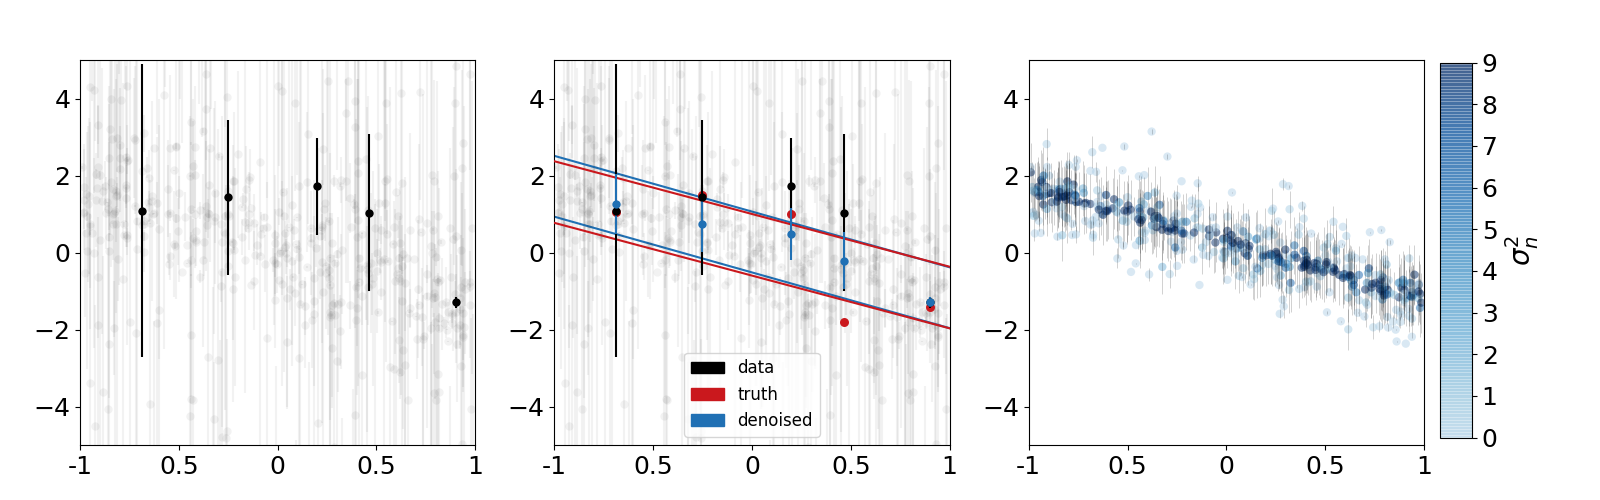
\includegraphics[width=\textwidth]{toy.png}
\caption{ {\bf Why does this work}: An example of generating posterior beliefs of true values from noisy data by using the noise-deconvolved distribution of data as a prior. The upper left panel visualizes the simplified toy distribution. The red lines are the $1\sigma$ contours of the distribution, and the red points are 1024 samples from the distribution. These same $1\sigma$ contours are drawn in the bottom left panel. In the upper right and lower left panel, the grey points are these same 1024 samples of the distribution but with some measurement uncertainty added to them. The error bars show the $1\sigma$ measurement uncertainties. The black points are 5 randomly chosen data to highlight the method. In the lower left panel, the blue lines represent the noise deconvolved, best estimate for the underlying distribution. The blue points represent the posterior belief of the true values of the noisy black points using the noise deconcolved distribution as the prior. The red points represent the actual true values. The lower right panel shows the posterior belief of the true value for all the points. They are colored by the measurement uncertainty, showing that data with larger measured variance are more influenced by the prior and lie towards the center of the noise deconvolved distribution, or prior. In contrast, more certain measurements tend to lie closer to their measured value. The blue points are better than the black for doing stuff.}
\label{fig:toy}
\end{figure}

In this paper we use the noise deconvolved observed \cmd\ as a prior to infer more precise parallax pdfs from \gaia\ measurements.
Understanding this method is challenging because we are using the data both for the prior and the likelihood in our inference.
To ease understanding, here we will demonstrate this method with a simpler toy model.
Instead of inferring more precise parallax pdfs using the 2D distribution of the \cmd\ as our prior, for this simpler model we will infer more precise pdfs of the value $Y$.
We will do this simpler inference using a prior that is also a 2D distribution: a 1D Gaussian in the y-direction, with a running mean $\mu = mx + b$ and some thickness $t$.
Here the thickness of the distribution mimics the true thickness of the \cmd\ due to age, mass and metallicity.
The $1\sigma$ contours as well as (noise free) samples from the toy model distribution are shown in Figure \ref{fig:toy}, upper left panel.
Similarly, noisy samples from this distribution are shown in the upper right panel.
Using a representation of the true distribution (which we learn from the noisy data) as our prior, we can infer some posterior belief of $y_{\true,n}$, a true sample of the distribution, from $y_n$, a noisy sample of the distribution.

Setting up the problem in more detail, we have the true underlying distribution of points and the noisy data

\begin{eqnarray}
y_{\true, n} \, &=& \, m_{\true}\,x_n + b_{\true} + \Delta_n \\
y_n \, &=& \, y_{\true,n} + \epsilon_n
\label{eq:ytrue}
\end{eqnarray}

where $\Delta_n$ is drawn from the Gaussian function $\mathcal{N}(\Delta_n \given 0, t^2)$, and $\epsilon_n$ is drawn from the Gaussian function $\mathcal{N}(\epsilon_n \given 0, \sigma_n^2)$, so $\sigma_n$ is the measurement uncertainty.
These represent true and noisy draws from a distribution that is a straight line with some thickness $t$, and are visualized in the upper panels of Figure \ref{fig:toy}
The upper left shows 1024 realizations of the true values, and the upper right, as well as lower left, show 1024 realizations of the noisy values $y_n$ and their associated measurement uncertainties $\sigma_n$ as the grey points. Here we highlight 5 random points in black to highlight the method, but the same method is being applied to all the data.

To infer a pdf of the true y value for each measured y value we need a prior. For our prior we will use an estimate of the underlying true distribution that the noisy data $y_n$ are drawn from, which we build from the noisy y data themselves.
We learn the noise-deconvolved function using marginalized maximum likelihood estimation (MML), which marginalizes over the true data values (we never need to know them) and maximizes the likelihood of the data. Here our likelihood for each individual datum is

\begin{equation}
p(y_n \given m, b, t^2, \sigma_n^2) = \mathcal{N}(y_n \given m\,x_n + b, t^2 + \sigma_n^2)
\label{eq:toyLike}
\end{equation}

It is a Gaussian because the noise model is a Gaussian. The likelihood of the full data set is then the product of the individual likelihoods

\begin{equation}
\prod_n\, p(y_n \given m, b, t^2, \sigma_n^2).
\label{eq:toyLikeFull}
\end{equation}

Maximizing this joint likelihood of all the data is the same as minimizing

\begin{equation}
\chi^2 = \sum_n \frac{[y_n - [m\,x_n + b]]^2}{[\sigma_n^2 + t_n^2]} + \sum_n\,ln(2\pi\,[\sigma_n^2 + t^2])
\label{eq:chisq}
\end{equation}

This MML gives us the best fit parameters $\hat{m}$, $\hat{b}$, and $\hat{t}$. In Figure \ref{fig:toy}, lower left panel, the true functions $y_{\true} = m_{\true}\,x + b_{\true} \pm t_{\true}$ are shown as the red lines, and the best fit MML functions $\hat{y}_{\true} = \hat{m}\, x + \hat{b} \pm \hat{t}$ are shown as the blue lines. Now that we have an estimate of the true underlying distribution $\hat{y}_{\true}$, we use this as a prior to infer a posterior belief of the true values for each datum $p(y_{\true,n} \given y_n, \tilde{\sigma}_n^2)$.

Here is a good point to step back and acknowledge that our method is odd/strange/different/new (which maybe you're also currently thinking but can't quite express why yet). We are using the set of data to determine the noise-deconvolved distribution, and then using that noise-deconvolved distribution to make inferences on the data. We are technically using the data twice! If we were going to be fully, technically correct, we should learn the distribution, but leave one datum out; the one datum we want to infer the true y value for\footnote{DWH: Remember what this brain dump is for}. Leaving one datum out to estimate the prior and then inferring the posterior for that datum is way too expensive for the 1024 points in our toy model, and also for the 1.2 million stars in our actual data set. Luckily with large data sets, even at 1024, 1 datum is $\sim0.1\%$ of your dataset and therefore leaving that point out will not change the MML parameters of your noise-deconvolved distribution, and with the \gaia\ dataset of over a million stars, we can safely step into the Empirical Bayes regime. (Talk more about emperical bayes here?)

So using Bayes theorem
\begin{eqnarray}
p(y_{\true,n} \given y_n, \tilde{\sigma}_n) &=& p(y_n \given y_{\true,n}, \sigma_n)\,p(y_{\true,n}) \\
p(y_n \given y_{\true,n}, \sigma_n) &=& \mathcal{N}(y_n \given y_{\true,n}, \sigma_n) \\
p(y_{\true,n}) &=& \mathcal{N}(y_{\true,n} \given \hat{m}\, x_n + \hat{b}, \hat{t})
\label{eq:toyBayes}
\end{eqnarray}

Since everything is Gaussian, this can be done analytically by multiplying Gaussians together. In Figure \ref{fig:toy} lower left panel, the blue points represent the posterior belief of the true value $p(y_{\true,n} \given y_n, \tilde{\sigma}_n)$ for the highlighted black points. The red points are the true y values.
The blue points in Figure \ref{fig:toy}, lower right panel, show the expectation value and $1\sigma$ uncertainty of the posterior belief for all 1024 $y_n$.
When the true values are inferred in this way, the associated variance $\tilde{\sigma}_n^2$ is the convolution of the true distribution variance $t^2$ and the measurement variance $\sigma_n^2$.
The points are colored by their measurement variance $\sigma_n^2$ which shows that noisier measurements are more influenced by the prior and get pulled closer to the center of the MML distribution, our prior. In contrast, more certain measurements remain closer to their measured values $y_n$.
By inferring the true y value from the measured y value in addition to the prior information of the distribution the y value was drawn from, this we have better estimates of the true y value for each point. Bringing the toy model back to our original problem, using the noise-deconvolved CMD as our prior allows us to get better estimates of the parallax for each star.

\section{Assumptions and methods}

We make the following assumptions. The method we present is correct
and justifiable under these assumptions, each of which is questionable
in its own right. We return to criticize these assumptions---and the
method that flows from them---in the Discussion below.
\begin{description}
\item[stationarity] We make an assumption of \emph{stationarity}; that is, that the
  stars measured at lower signal-to-noise have analogs measured at
  higher signal-to-noise.  In detail, this assumption is wrong, of
  course (for example, distant halo stars are different than local
  disk stars), but the stationarity assumption is fairly weak; as long
  as there is support in the high signal-to-noise stars for the types
  of stars seen at low signal-to-noise, the results will not be
  strongly biased, but this assumption is deep and fundamental to this
  work.
\item[big data] We assume that we have large numbers of stars, large enough that
  an empirical-Bayes or maximum-marginalized likelihood is a safe
  approximation to full Bayesian inference. This assumption will be
  least true in the least-populated parts of the \cmd. In the extreme
  case of a stellar type with only one (statistically distinct)
  exemplar in the data set (for example, a white dwarf), this assumption will be maximally wrong.
\item[noise model] We assume that the \tgas\ parallax uncertainties dominate the
  noise in any estimates of absolute magnitude. We further assume that
  the parallax and color uncertainties are Gaussian in form with
  correctly known variances. In detail, we assume that the [INSERT
    CORRECT TERMINOLOGY FROM GAIA HERE] parallax uncertainty estimates
  are correct. Here we are making use of the fact that, for
  de-noising, under-estimation of measurement noise is conservative
  (it leads to under-deconvolution).
\item[dust] We treat the \panstarrs-based three-dimensional dust maps (\citealt{green15})
  as correct in their median dust estimates, and their
  effects on color and magnitude. As we optimize the empirical-Bayes model, we iteratively update each star's
  dust correction at its updated, inferred distance. Our assumption is that these corrections are
  good enough, and uncertainties in these are not dominant, for either
  color or absolute magnitude.
\item[mixture of Gaussians] We assume that the \cmd\ can be represented with a mixture of
  Gaussians in a particular transformed space. This mixture we fix
  (with only heuristic analysis) at 128, 512, and 2048 Gaussians in
  different experiments.
\item[no physics] We make no use of stellar models; our only assumptions about
  stellar physics are generic and implicit (for example, that the
  \cmd\ is somehow smooth and compact).
\end{description}

\subsection{Setting up the Inference}
 \emph{Think about presentation, prioritizing/highlighting prior but logically building it from an full inference perspective and needing a prior, then dive into prior stuff. It's confusing right now jumping between inference and prior building !!}

Under these assumptions, we would like to infer the true parallax $\varpi_{\true}$ for each star given its measured parallax $\varpi$ and associated uncertainty $\sigma_{\varpi}$ from \tgas.
The strength of our inference method here lies in how we generate our prior information on the true parallax.
Supplementary to the trigonometric measure of distance, the photometry of stars is also informative of their distances.
The intrinsic temperatures and luminosities of stars tightly correlate leading to the observed colors and absolute magnitudes of stars also tightly correlating, usually visualized as the color--magnitude diagram (\cmd).
The tight correlation of the \cmd\ benefits our inference because the luminosity or absolute magnitude of a star, when compared with its brightness or apparent magnitude, contains distance information.
We include this distance information in the inference of the true parallax by using the \cmd\ as our prior.
Specifically, we use the \cmd\ generated from the data themselves as our prior.
Instead of assuming a functional form for the spatial distribution of stars in the Milky Way (\citealt{astraatmadja16b}), or relying on stellar models (\citealt{gaia16}), we build a noise-deconvolved estimate of the \cmd\ from the observed colors and absolute magnitudes of our full set of stars.
This \cmd\ model becomes, for each star---given its observed color and magnitude (and uncertainties on those)---a prior pdf for the distance to that star.

Because our prior is the \cmd, our inference will include not only the parallax from \gaia, but also the photometry of the stars. For inferring the true parallax, including generating our \cmd\ prior, we use the $J$ and $K$ band photometry from \tmass, as well as the parallax from \gaia. Our true, latent values are the $(J-K)^{true}_n$ color and the $J$ band absolute magnitude $M^{true}_{J,n}$ for each star, which we encapsulate in the true vector $\mathbf{Y}$. The observed data is the dust corrected color $(J-K)^c_n$, the \gaia\ parallax $\varpi_n$ in units of $[mas]$, and the dust corrected $J$ band magnitude $J^c_n$, which we encapsulate in the data vector $\mathbf{y}$. Instead of transforming the parallax and apparent magnitude into an absolute magnitude, the data vector $\mathbf{y}$ contains a transformation of the dust corrected absolute magnitude

\begin{equation}
y_0 = \varpi\,10^{0.2J^c_n} = 10^{0.2\,M^c_{J,n} + 2}
\label{eq:transform}
\end{equation}

The transformation of the dust corrected absolute magnitude, Equation \ref{eq:transform}, is required to to keep the uncertainties Gaussian, which, under some assumptions along with this transformation, we maintain. Gaussian uncertainties are required to generate our prior using \xd\, but more about this and our dust corrections below.
Our prior assumptions $I$ are the uncertainties in each of these measurements, as well as the Greene dust map. So our full terminology is

\begin{equation}
\begin{aligned}
\mathrm{true \, vector} \quad &\mathbf{Y}_n = [10^{0.2\,M^{true}_{J,n} + 2}, (J-K)^{true}_n] \\
\mathrm{data \, vector} \quad &\mathbf{y}_n = [\varpi_n\,10^{0.2J^c_n}, (J- K)^c_n] \;  n \in \mathrm{stars} \\
\mathrm{with \; apparent \; magnitude} \quad &J^c_n = J_n - Q_J\,E(B-V)_n \\
\mathrm{and \; color} \quad &(J - K)^c_n = J_n - K_n - Q_{JK}\,E(B-V)_n \\
\mathrm{assumptions} \quad &I_n = \left\{\left\{\sigma^2_{\varpi, n}\right\}, \left\{\sigma^2_{J,n}\right\}, \left\{\sigma^2_{K,n}\right\}, \mathrm{Dust \, Map}\right\}
\end{aligned}
\label{eq:data}
\end{equation}

where $E(B-V)_n$ is the output of the Green et al dust model, and $Q_{\lambda}$ is the correction factor for a photometric band assuming some reddening law.

If life were simple, our inference would be a 1D problem using Bayes theorem and look something like:
\begin{equation}
p(\varpi_{\true} \given \varpi, \sigma^2_{\varpi}) = \frac{1}{Z}\,p(\varpi \given \varpi_{\true}, \sigma^2_{\varpi}) \, p(\varpi_{\true}) \quad ,
\label{eq:bayes}
\end{equation}
where $p(\varpi \given \varpi_{\true}, \sigma^2_{\varpi})$ is the likelihood of the observed parallax, $p(\varpi_{\true})$ is a prior probability density (pdf) for the
parallax, and $Z$ is a normalization constant.

But life isn't simple, and our prior is a 2D function in color and transformed absolute magnitude space, so our full inference in done in 2D space as well.
We assume (as \gaia\ suggests) that the parallax likelihood is Gaussian, as well as the $(J-K)^c_n$ color likelihood. So our full likelihood of the data is
\begin{equation}
p(\mathbf{y}_n \given \mathbf{Y}_n, I_n) = \mathcal{N}(\mathbf{y}_n \given \mathbf{Y}_n, V_n)
\end{equation}

with \\
$V_n = $
\[
\begin{bmatrix}
\sigma_{J,n}^2 + \sigma_{K,n}^2 & 0 \\
0 & (\sigma_{\varpi}\,10^{0.2\,J_n^C})^2
\end{bmatrix}
\]


where $\mathcal{N}$ is a 2D Gaussian function with mean $\mathbf{Y}$ and variance $V_n$.
Here we have assumed that the parallax uncertainty is significantly larger than the $J$ band uncertainty, and therefore the dominant uncertainty in the transformed absolute magnitude, so we take $J_n^C$ as a point estimate and only propagate the parallax uncertainty. This is to keep our uncertainties Gaussian so we can use \xd\ generate our prior below.

This likelihood is the probability of the data vector given the true vector, but we
want to flip it around and infer the true vector and therefore the true parallax, or distance. We do this
analogous to Equation \ref{eq:bayes}.


\begin{equation}
p(\mathbf{Y}_n \given \mathbf{y}_n, I_n) = p(\mathbf{y}_n \given \mathbf{Y}_n, I_n) \, p(\mathbf{Y}_n)
\end{equation}

where $p(\mathbf{Y}_n)$ is our prior.

\subsection{Generating the Prior}

To generate our prior, we fit the data in the slightly transformed \cmd\ space, using Equation \ref{eq:transform} instead of absolute magnitude. We fit this transfromed \cmd\ using \xd\ which deconvolves the data with its uncertainties, which are heterogeneous measurement uncertainties. It generates the underlying distribution from which the uncertain data were drawn from. \xd\ generates a represention of the distribution as a mixture of Gaussians which maximizes the marginalized likelihood of the data, marginalizing over the true data.

\xd\ generates the gaussian parameters

\begin{eqnarray}
\alpha &=& \left\{\mathrm{amp}_k, \mu_k, V_k\right\}_{k=1}^K \; k \in \mathrm{Gaussians} \nonumber\\
       &=& \argmax_{\alpha} \, \Pi_n \, p(\mathbf{y}_n \given \alpha) \nonumber\\
       &=& \argmax_{\alpha} \, \Pi_n \, \int p(\mathbf{y}_n \given \mathbf{Y}_n) \, p(\mathbf{Y}_n \given \alpha)\mathrm{d\mathbf{Y}_n}
\label{eq:xdmml}
\end{eqnarray}

where $\alpha$ encapsulates the parameters of each Gaussian in the mixture of Gaussians that defines our \cmd\ prior.

\subsection{Back to the Inference}

To infer $\varpi_{\true}$ we first do the inference in the 2D space of the \cmd

\begin{equation}
p(\mathbf{Y} \given \mathbf{y}, \alpha) = \frac{1}{Z} \, p(\mathbf{y} \given \mathbf{Y}) \, p(\mathbf{Y} \given \alpha)
\label{eq:posterior}
\end{equation}

We then project the 2D posterior into the 1D transformed absolute magnitude space, and do a little algebra to get

\begin{eqnarray}
p(\mathbf{Y}_0 \given \mathbf{y}, \alpha) &\rightarrow& p(\varpi_{\true} \given y, \alpha) \, f(\varpi_{\true}) \\
f(\varpi_{\true}) &=& \begin{cases}
              1 \quad \mathrm{if} \quad -2 < \mathrm{log}_{10} \varpi_{true} < 2\\
              0 \quad \mathrm{otherwise}
              \end{cases}
\label{eq:parallaxPost}
\end{eqnarray}
with $f(\varpi_{true})$ being a window function to insure the true parallax is positive and put it on a similar grid for all the posteriors.
And with a jacobian this becomes a posterior on distance.

Crossvalidation?

\section{Data and results}
\begin{figure}
\centering
  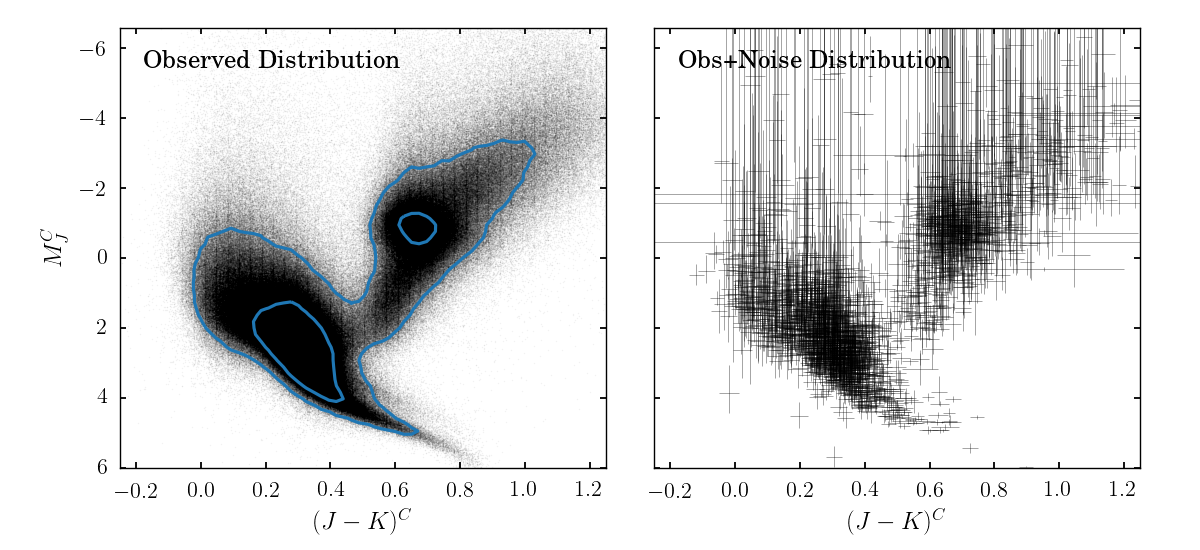
\includegraphics[width=\textwidth]{data.png}
\caption{The observed \cmd: To visualize the full dataset, in the left panel we use the point estimates of the \tmass\ $J-K$ color, the $J$ band apparent magnitude, and the \gaia\ parallax. The blue lines represent the $1\sigma$ and $2\sigma$ contours for the distribution. To give a sense of the uncertainties, in the right panel we subsample the dataset and include the $1\sigma$ uncertainties. The uncertainties are dominated by the parallax noise, with many stars diverging to infinitely far away and therefore very intrinsically bright.}
\label{fig:data}
\end{figure}

We use stars crossmatched in \tgas\ and \tmass\, and lie within the observing footprint of \panstarrs\ to access the Greene 3D dust model. We require the photometry have real values, and nonzero, real errors, and remove a small selection of \tmass\ stars that have zero color and zero J band magnitude.

\subsection{Dust}

\begin{figure}
\centering
  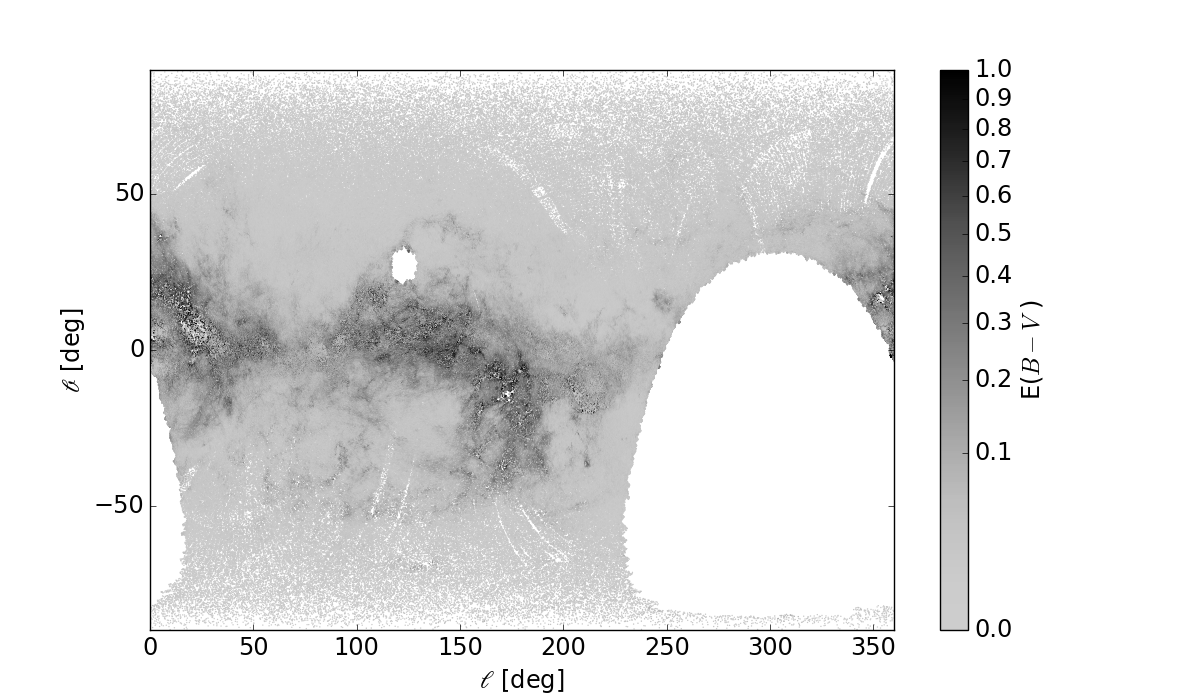
\includegraphics[width=\textwidth]{dust.png}
\caption{The converged dust values at the 5\% distance projected on the l,b galactic coordinates. This shows both the footprint of our analysis as well as the dust values we used. Each point represents a single star in our cross matched catalog. The large missing areas are due to the lack of dust values from \panstarrs\ since it only looked above -30 degrees in dec }
\label{fig:dust}
\end{figure}


We correct for dust using 3D Bayestar (Schlafly+Finkbeiner) with an estimate of the distance from iteratively sampling our posterior distances. Dust corrections are non trivial for stars with poor signal to noise. Stars with poor signal to noise have a likelihood that is consistent with infinite distance and can therefore have severe dust corrections. This is most obvious in the giant stars, which tend to have the lowest signal to noise, and can therefore have dust corrections $> 2$ magnitudes. To apply a dust correction to the \tmass\ photometry, we first generate our prior using the observed, attenuated photometry. Using this raw prior we infer more precise distances to all the stars in our sample. We then use this more precise distance posterior to get a measurement of dust in the 3D dust map. This approach minimizes severe distances from the likelihoods alone and their associated severe dust corrections. In detail, we take the $5\%$ quantile of each distance posterior, so the closest bit of the posterior, and sample the Green et al 3D dust map at that distance. We take the $5\%$ quantile, as apposed to the median for example, to do a light dust correction because over correcting for dust can shoot the likelihood into an unphysical, different space of the CMD and then bias the distance inference. For each distance we sample the median of the probabilistic dust model. We apply each light dust correction to our \tmass\ photometry given by Equation \ref{eq:data} where $Q_{\lambda}$ = [0.709, 0.302] for bands [J, K] respectively, taken from table (REF TABLE SFD), and $E(B-V)$ is the output of the Green et al dust models. We then regenerate our prior using the lightly dust corrected photometry. We do not update the errors, but keep them the same as before the dust correction, which is wrong and under representing our errors but this leads again to a lighter deconvolution. We could add the covariance of the dust to our likelihoods, but this is beyond the scope of this demonstration of concept. We iterate this process 10 times, however the dust values seem to converge after about 2-3 iterations. The iterative process allows for slight variations in distance and corresponding dust to become more consistent with the \cmd.

Should I quote some statistics about the dust corrections? mostly small? maybe difference before/after applying prior to distance?

\subsection{Prior}

\begin{figure}
\centering
  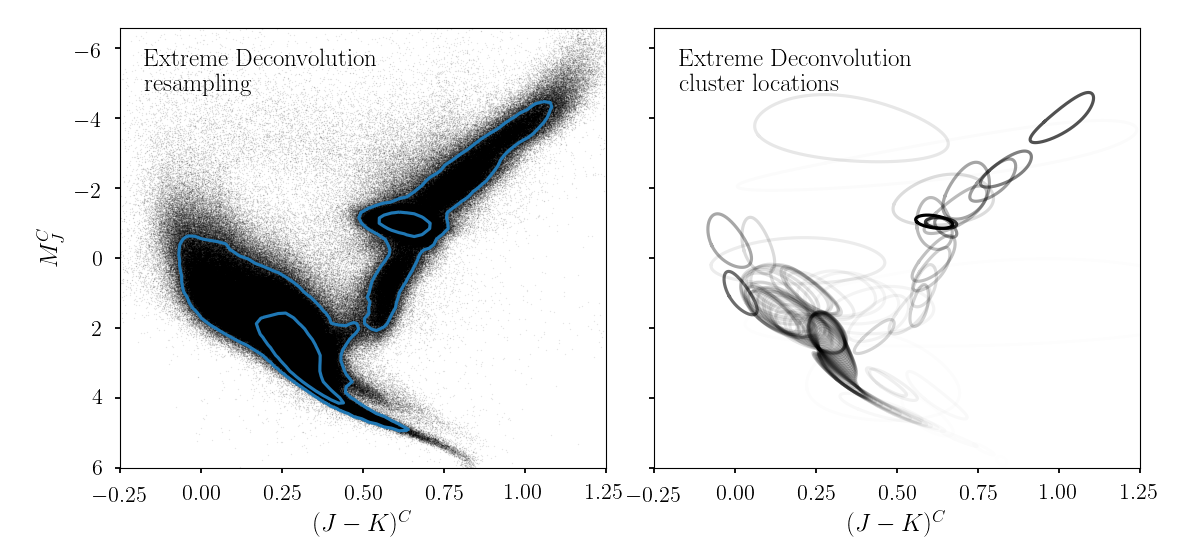
\includegraphics[width=\textwidth]{prior_ngauss128.png}
\caption{Prior: the XD generated mixture of gaussians we use as our prior. The left panel shows a sampling of the prior, which is a mixture of gaussians shown in the right hand panel. The blue lines are the $1\sigma$ and $2\sigma$ contours. The gaussians have a funny shape due to the transformed space in which we fit the data.}
\label{fig:prior}
\end{figure}

\begin{figure}
\centering
  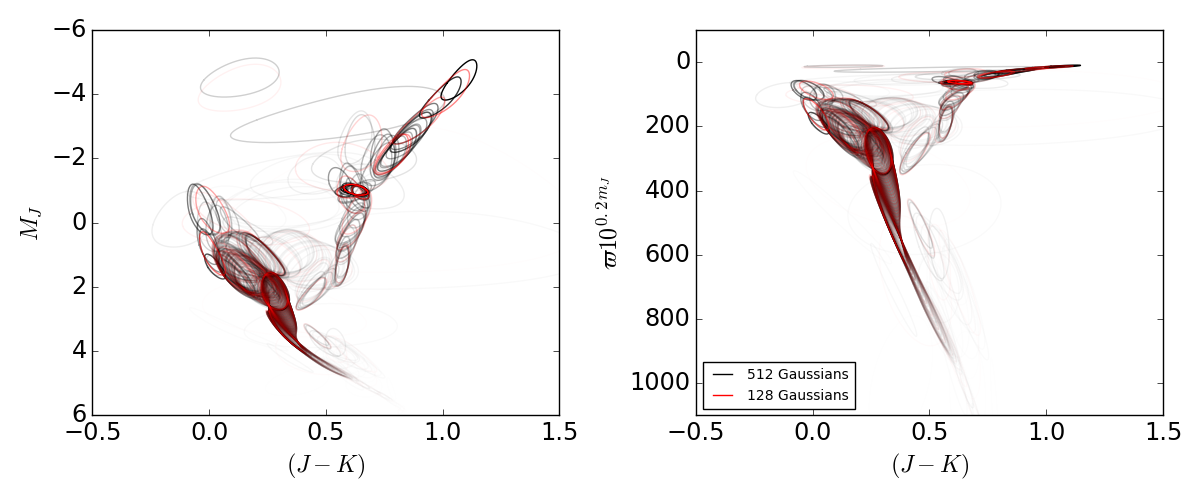
\includegraphics[width=\textwidth]{priorNgaussComparison.png}
\caption{Prior: the XD generated mixture of gaussians we use as our prior. To determine the number of gaussians we used cross validation, using 70\% of our sample as a training set and 30\% as the test set. Increasing the number of gaussians we used continued to increase the likelihood of the test set of data, showing that we are no over fitting. Using more gaussians as our prior did not substantially change our posterior results, but it did start to highlight the features of the CMD.}
\label{fig:priorCompare}
\end{figure}




\begin{figure}
\centering
  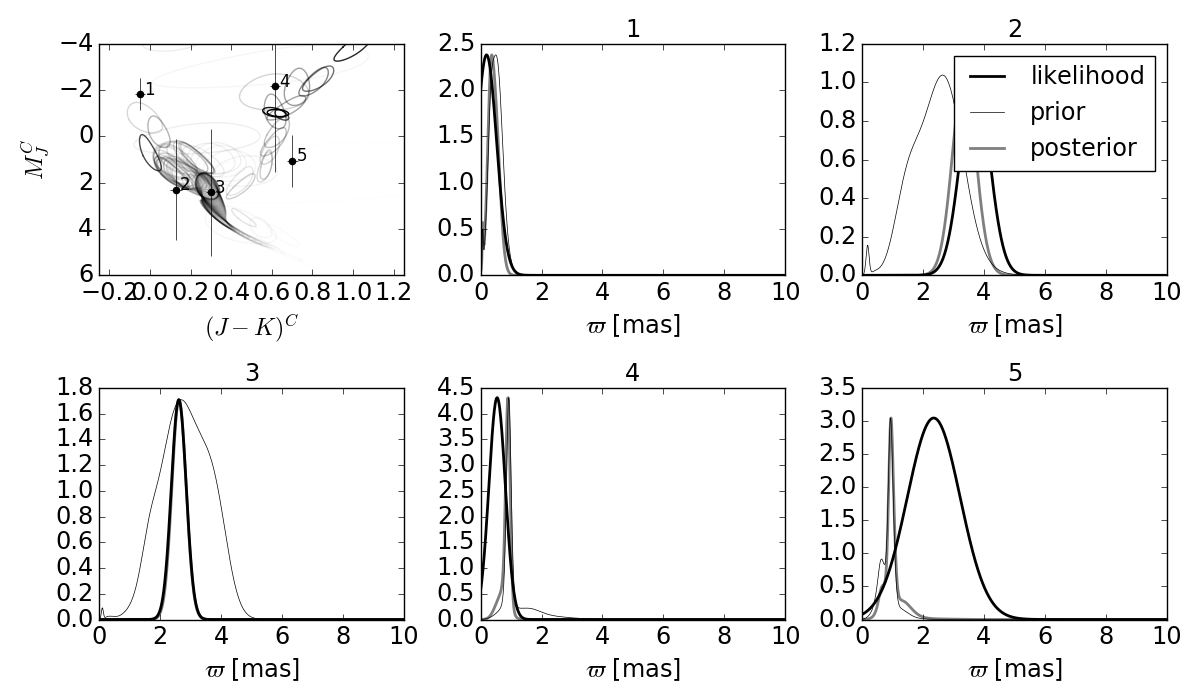
\includegraphics[width=\textwidth]{posterior.png}
\caption{5 example posteriors showing the priors and likelihoods as well}
\label{fig:posterior}
\end{figure}


\begin{figure}
\centering
  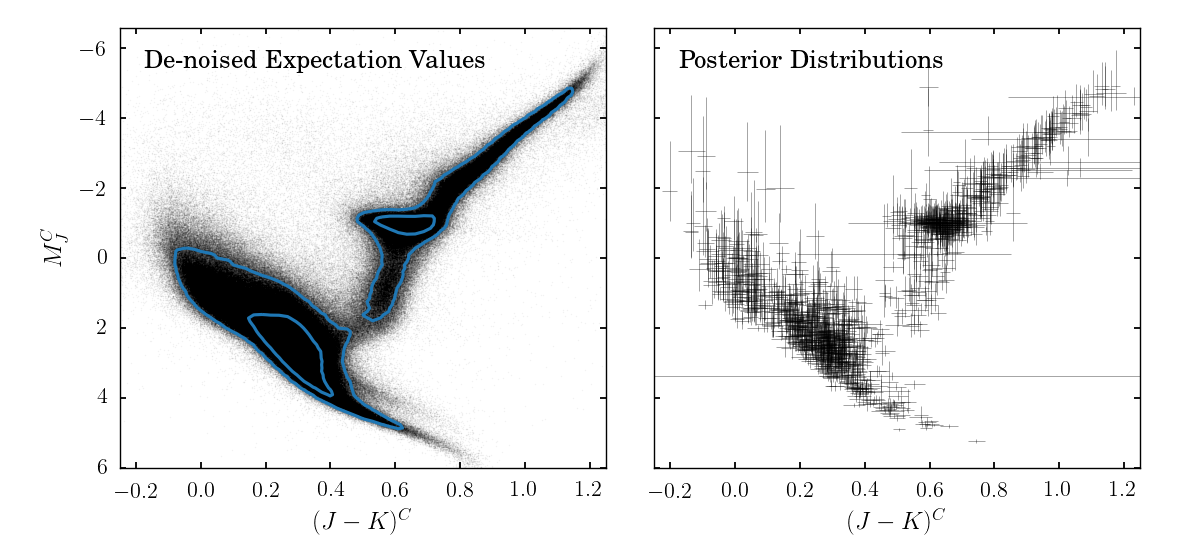
\includegraphics[width=\textwidth]{posteriorCMD.png}
\caption{the expectation values and subsampled error bars. Notice that some parts of this \cmd\ are tighter than the prior, or noise-deconvolved \cmd. The visual of the prior is a sampling of the Gaussians, but this is the expectation value so this lies much closer to the center of the distribution. Similar to the toy model, where the pdf maximum of the noisier points lies in the center of the distribution.}
\label{fig:posteriorCMD}
\end{figure}


\begin{figure}
\centering
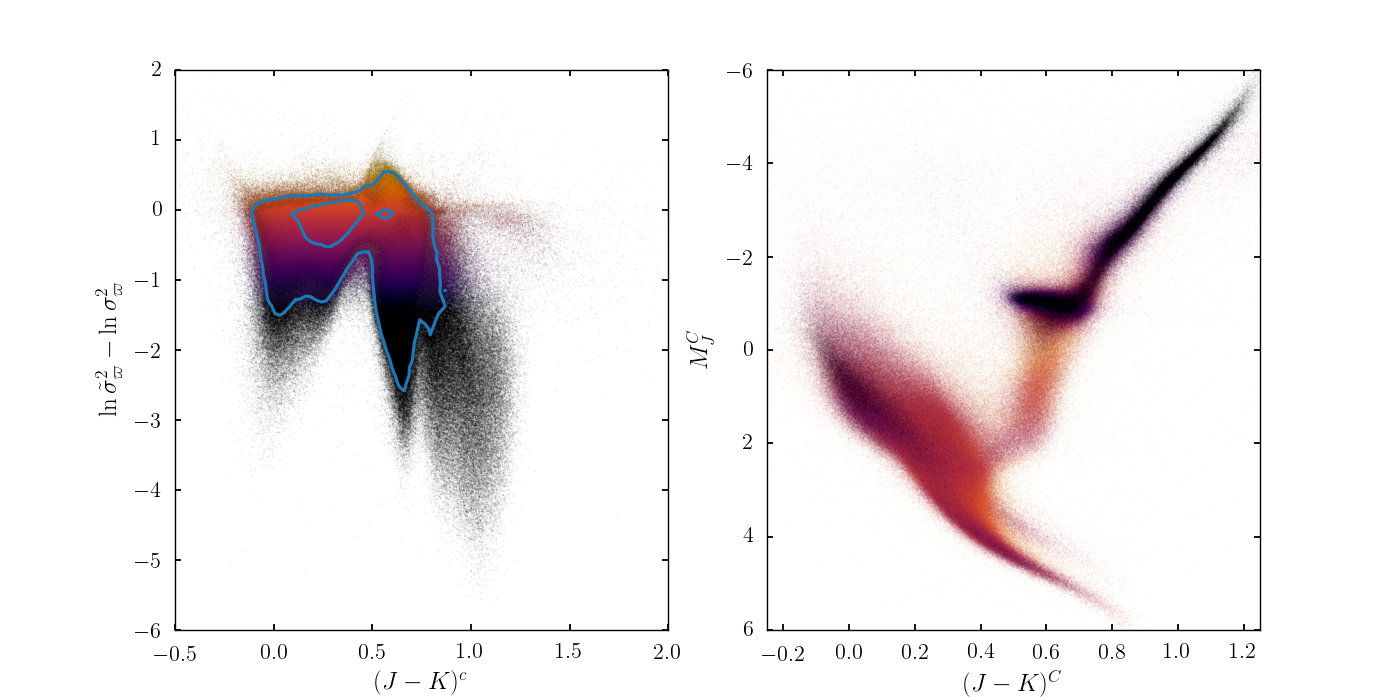
\includegraphics[width=\textwidth]{delta.png}
\caption{Fractional Change in Variance: The left panel shows the natural log of the fractional change in the variance of the posterior relative to the likelihood as a function of the stellar color. The coloring of the points in both panels is by the fractional change in variance to guide the coloring of the right panel. The blue lines are the $1\sigma$ and $2\sigma$ contours. The median fractional change is XXX. Some posteriors have significantly smaller variances shown in black, but some actually increase in variance, shown as the yellow bump at $(J-K)^C$ about XXX. The right panel shows the posterior point estimates on the CMD colored by fraction change in variance. There is significant changes for the red giant branch stars, as well as some main sequence stars.}
\label{fig:delta}
\end{figure}


\subsection{Results: Distances to M67}
\begin{figure}
\centering
  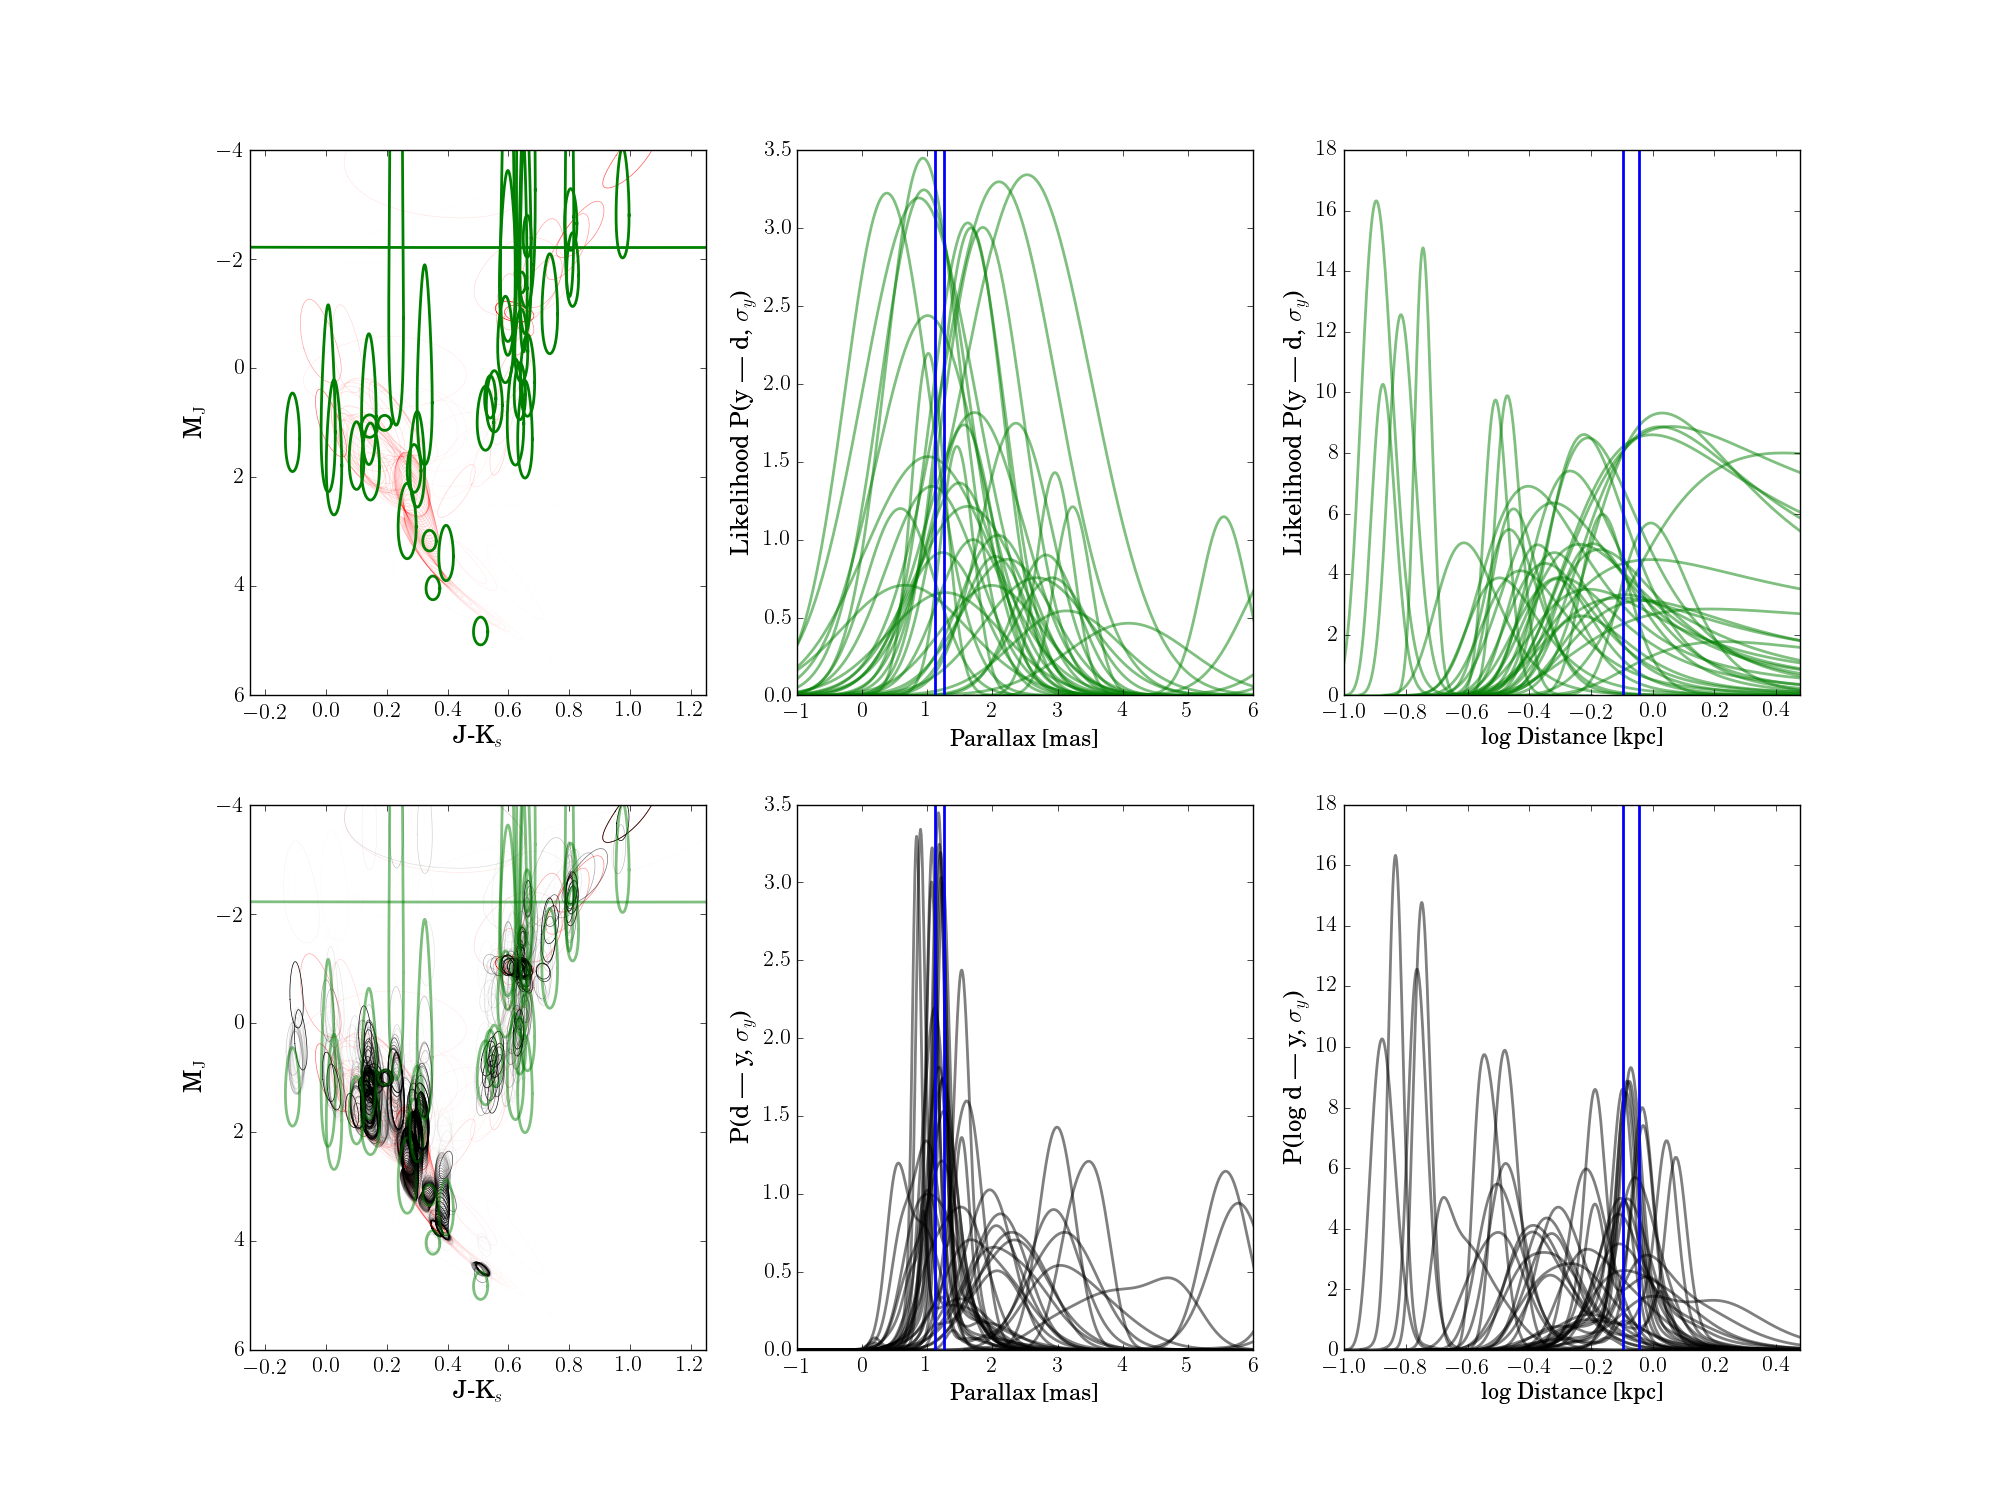
\includegraphics[width=\textwidth]{distancesM67.png}
\caption{Proof of concept: parallax inference to the open cluster M67}
\label{fig:m67}
\end{figure}

As proof of concept we inferred the distances to stars in the open cluster M67. It is an open cluster in the constellation Cancer and is estimated to be 3-5 billion years old and 800-900 pc away. Previous work (cite CBJ) has estimated that bad things happen if you try to infer a distance as the inverse of the observed (noisy) parallax when the signal to noise of the parallax measurement drops below 5. With \gaia\ parallaxes having a minimum uncertainty of about 0.3 mas, the SN reaches 5 for the most certain parallax measurements at about 700 pc, right where this cluster lies. So it is a great test case for comparing parallax inferences with or without a prior. We made a window of 1 square degree on the sky with the cluster M67 lying in the middle. The cluster is visibly obvious as a clustering of stars in a visualization of the \gaia\ data on the 2D sky. With our converged dust values, and it's associated prior, we calculate the posterior of the true parallaxes to the stars within this window on the sky around M67. Figure \ref{fig:m67} shows the comparison of the likelihoods and posteriors. The vertical lines bracket the parallaxes of, or distances to, the cluster. The likelihoods of the observed parallaxes, shown in the top row, are broad and the cluster is not obvious at all. The posteriors, shown in the bottom row, show a sharp peak in the probability at the previously determined distance to the cluster, the vertical lines, for far more stars than the likelihoods would imply. Our prior is not only making parallaxes more precise but also (possibly) increasing the accuracy. Too strong?


\subsection{Output data}
DWH: Placeholder for the output format for our data products.
RA, DEC, l, b, tgas source ID, tycho-2 source ID, parallax samples, parallax posterior, flag (some fraction of posterior not in window, negative gaia parallax, ...)

\section{Discussion}

We have shown that it is possible to obtain photometric parallaxes for
distant stars in the \gaia\ \tgas\ data without any use of physical stellar
models, nor models of the Milky Way.
That is, the geometric parallaxes can calibrate a set of photometric
models that are purely statistical---a model of the data rather than
a model of stars \foreign{per se}.
This opens up the possibility of completing the goals of the \gaia\ Mission
without building in unnecessary assumptions about the mechanical properties
of stars or the Galaxy.

We obtained the photometric parallaxes in this project
by building a data-driven model of the
color--magnitude diagram (\cmd) of the stars in the \tgas\ data set,
and using it as a prior pdf for Bayesian interences.
The posterior pdfs for distance that we obtain are, in general, much
narrower than the likelihood functions delivered by the
\gaia\ Mission, and therefore the distance estimates (or,
equivalently, parallax estimates) are much more precise.
It is not surprising that a Bayesian inference provides more
precise inferences than the likelihood function alone; Bayesian
inferences bring in new information that decrease variance (but
often introduce bias).
We have shown that, in addition to pure precision improvements, at
least some aspects of \emph{accuracy} have been improved as well, by
showing that the posterior distance estimates to stars in stellar
clusters [HOGG: Is this too general?] are much more clustered than likelihood-based distance
estimates.

Although we have not performed principled hierarchical Bayesian inference in this
project, we built our prior for each star's distance by
performing a statistically responsible deconvolution
of the \gaia\ \tgas\ data that is justifiable under a clear set of
assumptions.
This deconvolution makes use of a reasonable noise model and an
assumption of stationarity to shrink the parallax uncertainties, and
do so dramatically for the stars measured at lower signal-to-noise.
Because the method we use (Extreme Deconvolution or \xd, which is
an Empirical Bayesian maximum-marginalized-likelihood estimator) accounts for
heteroskedastic noise, we were able to build our photometric parallax
model---which is a model of the \cmd---using
all the data, not just the data with the highest signal-to-noise or
largest parallaxes.
That is, the model for the \cmd\ we have built is representative for
(a subset of) the \tgas\ Catalog.
Inasmuch as that is true, we expect any (sensible) distance estimates
we generate from our distance posterior pdfs to be only weakly biased.

The Empirical Bayesian methodology is a good approximation to full
hierarchical inference in the limit of large numbers of data points.
That is, when no individual star is carrying a lot of weight in the
model of the \cmd.
With its millions of stars, the \tgas\ Catalog may appear to safely
live in this limit.
However, because there are parts of the \cmd\ that are poorly populated,
even in \tgas, the Empirical Bayes approximation may be bad for some
color ranges.
In particular, there appear to be essentially no white dwarf stars,
and other classes (like bright red giant branch stars) have few to no exemplars
in the data set at high signal-to-noise (in parallax).
For all these reasons, we do think that this approximation is not perfectly
safe, and it is a goal to explore full hierarchical modeling in the coming
years (and see, for example, Leistedt et al. in preparation).

In some sense, the biggest limitation of the data-driven \cmd\ model
created in this project is that we made no use of any kind of \tgas\ selection
function or completeness estimate or inverse-selection-volume corrections.
That is, the model is a model of the \tgas\ Catalog
(or really the \tgas--\tmass\ intersection), not of the stars in
the Milky Way, nor any volume-limited subsample of the Milky Way.
Importantly, because we used \emph{all} of the stars in the \tgas--\tmass\
intersection, the model \emph{is} representive of the full catalog,
even the distant parts, where all the parallaxes are measured at low
signal-to-noise.
This is in contrast to techniques that might build the model from only
the high signal-to-noise sources; such a model would be biased towards
stellar types and compositions found locally, lower-luminosity stars,
and stars which happened to get good parallaxes.
However, our use of the entire \tgas--\tmass\ intersection without
any selection function restricts the use of our \cmd\ model as a prior
to inferences within that same \tgas--\tmass\ intersection.
For example, it would be biasing to use this same prior to infer
distances for the full billion-star catalog released in \gaia\ DR1
alongside \tgas, or for stars fainter or brighter or bluer than those
included in the \tgas--\tmass\ intersection.

The outputs of this project include posterior pdfs and posterior
samplings for stellar parallaxes or distances.
It is tempting to treat these outputs as equivalent to some kind of catalog of
measurements, as we treated the original parallax measurements from \tgas.
That is, it is tempting to treat these as simply ``better'' measurements.
Taken one star at a time, this is permitted and true, and the basis for our
claim that we have de-noised the \tgas\ Catalog.
However, there are important differences, as there are with all
probabilistic catalogs (\citealt{hogg11}; \citealt{portillo17}), between the
measurements and the de-noised measurements.
The most important difference, for users of our output, between our
output and the \tgas\ data input, is that the \tgas\ data is the representation
of a likelihood function, whereas our ouptut is a
representation of a posterior pdf, one per star.
If used naively, posterior information can lead to serious statistical
errors, because each data point has had a prior multiplied in.
Multiplicative uses of the data will effectively take the prior
pdf to a large power.
We have (in previous work)
given examples of correct uses of posterior samplings or pdfs
for subsequent inferences (\citealt{hogg08}; \citealt{dfm14}); we
encourage power-users to consult those methodological
contributions before engaging with these outputs.

\subsection{Comparison with other priors}
\begin{figure}
\centering
  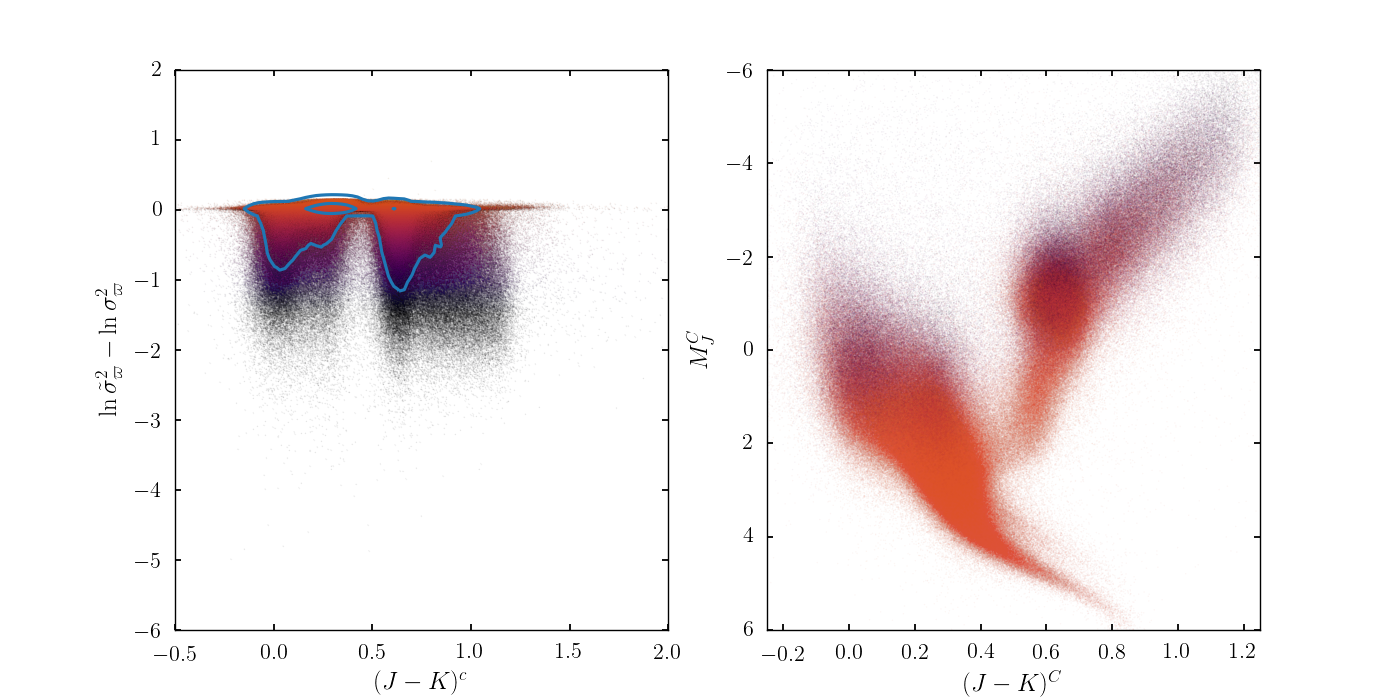
\includegraphics[width=\textwidth]{deltaSimple.png}
\caption{Other example prior: The same visualization as Figure \ref{fig:delta} of the change in the posterior, but here, if instead of prior information containing the \cmd\, the prior information is an exponentially declining spatial density of stars.  }
\label{fig:otherPrior}
\end{figure}

There are other prior information options when inferring distances to stars. One option is the exponentially declining spatial density of stars (cite: Tri, CBJ). It is parameterized by a scale length, and has the nice property that it is smooth out to very large distances so the posteriors are also very smooth. It is a fairly weak prior and basically sets a smooth scale at which it's challenging for stars to lie at, and also allows for negative parallaxes. It is a fairly broad prior so the median \gaia\ star has an increased posterior variance. It has the largest affect on the most noisy and negative parallaxes and has the nice property of bringing these noisy or negative measurements to reasonable parallaxes. Given this prior, what does the observed \cmd\ look like?  The \cmd\ is broad and the red clump highly stretched.


\subsection{What's That Feature?}
The denoised expectation values of the parallax projected into the \cmd\ show interest features.
\begin{itemize}
\item (1) Narrow Lower Main Sequence
\item (2) Wide Upper Main Sequence
\item (3) Plausible Binary Sequence
\item (4) Prominent Red clump
\item (5) Narrow Red Giant Branch
\item (6) Noticeable turn off
\end{itemize}
The lower main sequence is very narrow while the upper main sequence is much wider. This may be an age variation on the main sequence mixed with a malquist bias of only seeing a very small volume of lower main sequence stars but a much larger volume of upper main sequence stars. There is a plausible binary sequence of stars with about twice the brightness as the main sequence. The helium burning red clump is (surprisingly) prominent for the volume DR1 probed, and the red giant branch is straight/narrow. The main sequence turn off is noticeable and also surprisingly narrow, possibly a reflection of the star formation history of the local volume also mixed with a malmquist bias.

Come back to the assumptions. What happens if we change or violate them?

Long discussion of the noise model. We took serious short-cuts. Call out to Boris.

\subsection{Proper Dust Corrections}
Within our probabilistic framework, we improperly handle dust. We are taking a point estimate of the probabilistic dust model at a quantile distance of our posterior, correcting our photometry using this point estimate and rederiving the prior. A full, proper account would sample the dust model at distances sampled from the posterior and propagate those samples back into the prior during the iterative proccess. The issue, the reason we don't do a full probabilistic treatment, is that this proper dust distribution would not be a Gaussian distribution which \xd\ requires. We could calculate this more complex dust distribution and estimate it as a Gaussian distribution to feed to \xd, however, this is beyond the scope of this paper.


\subsection{Stationarity Assumption}
Stationarity assumes both the low and high signal to noise objects are being drawn from the same distribution, independent of noise. This isn't precisely true because most Gaia objects have similar noise $(\sim 3 mas)$, but their signal (parallax) depends on their distance. Nearby stars have higher signal (parallax) because they are closer and the nearby stars are mostly main sequence stars (IMF, timing, malmquist). However, we can see bright giants to much larger distances and therefore lower signal or parallax, leading to lower signal to noise. So the red giant branch is a population of relatively lower signal to noise objects compared with the main sequence. But I think this is ok, that the low and high signal to noise objects have to be drawn from the same distribution within some feature or patch of the space. This is all assuming the Gaia noise model is correct. If the uncertainties are over estimated then we could be over deconvolving (generating a tighter distribution than the truth) And in some extreme over estimate of uncertainties the lower signal to noise giants could be pulled to the main sequence. But with the quoted uncertainties this seems unlikely. As you move up the giant branch and probe farther giants the signal to noise will continue to diminish but I think this is okay since the color uncertainties are not large. Possibly a metallicity trend with distance, placing more nearby (higher S/N) objects at slightly different positions on the CMD pulling lower S/N objects to that distribution for our prior. But if something has small error bars is good data is good data both for inference and generating the prior

For very rare kinds of stars. Inference with our prior is bad for underrepresented populations in the \cmd. For example, it appears there are only $2$ white dwarfs in \gaia\ DR1. With them being very underrepresented in the prior, the amplitudes of the gaussians representing them is very small, so the WDs are more likely to be pulled to mimic a much farther away MS star.

\subsection{Cross Validation}
For generating our prior, we use a mixture of 128 Gaussians. This number, 128, was chosen heuristically. It makes the method computationally tractable, and is sufficient for this demonstration of concept, but more Gaussians might be desired for a more final data product. We would ideally use the optimal number of Gaussians determined by cross validation, but preliminary tests using cross validation suggest the optimal number of Gaussians is very large.

Compare with literature stellar models

How this compares to other Bayesian attempts at inferring distances,
like, eg, the Tri--Coryn papers. Favorably! And with \emph{fewer}
assumptions, in fact! What form should this comparison be in?

\acknowledgments It is a pleasure to thank
  Ana Bonaca (Harvard),
  Andy Casey (Monash),
  Dustin Lang (Toronto) for cross matched 2MASS-TGAS catalogue
  Jo Bovy (Toronto)
  Boris Leistedt (NYU)
  Adrian Price-Whelan (Princeton)
and the attendees at the Stars Group Meeting at the Flatiron Institute
Center for Computational Astrophysics for comments and input.
This project was developed in part at the 2016 \acronym{NYC} Gaia Sprint, hosted
by the Center for Computational Astrophysics at the Simons Foundation
in New York City.

This work has made use of data from the European Space Agency (\acronym{ESA})
mission \gaia\footnote{\url{http://www.cosmos.esa.int/gaia}}, processed by the Gaia
Data Processing and Analysis Consortium\footnote{\url{http://www.cosmos.esa.int/web/gaia/dpac/consortium}} (\acronym{DPAC}). Funding for the
\acronym{DPAC} has been provided by national institutions, in particular the
institutions participating in the Gaia Multilateral Agreement.

This publication makes use of data products from the Two Micron All
Sky Survey, which is a joint project of the
University of Massachusetts and the Infrared Processing and Analysis
Center/California Institute of Technology, funded by the National
Aeronautics and Space Administration and the National Science
Foundation.

This project was partially supported by This research was partially supported by
  the \acronym{NSF} (\acronym{AST-1517237}),
  \acronym{NASA} (grant \acronym{NNX12AI50G}),
  and the Moore-Sloan Data Science Environment at \acronym{NYU}.
It made use of the \acronym{NASA} Astrophysics Data System.
All the code used in this project is available online\footnote{\url{https://github.com/andersdot/stellarTwins}} under an open-source license.

%% \appendix
%% \section{Appendix material}

\bibliography{gaia}

\clearpage

\end{document}



%%
%% End of file `sample.tex'.
